\newpage
\section{ $C^0$ Interior Penalty Method for Biharmonic Equation}
\label{sec:ch1}


% \subsection{Hybrid DG Biharmonic Equation}%
% \label{sub:hybrid_dg_biharmonic_equation}

Let $\Omega \subset   \mathbb{R} ^2$ be a bounded polygonal domain and $\partial \Omega $ be its corresponding boundary.
\todo[inline]{ Why is this domain chosen to be polygonal? }
We can then define the fourth order problem as

\begin{equation}
\label{eq:bi_problem}
\begin{split}
    \nabla ^4 u - \beta \nabla ^2 u  + \gamma  & = f \quad \text{in } \Omega   \\
    \partial _{n} u & = 0 \quad \text{on } \partial \Omega  \\
    \partial _{n} \nabla ^2 u & = q \quad \text{on } \partial \Omega   \\
\end{split}
.\end{equation}
We will assume that $\gamma $ and $\beta $ is nonnegative constants, $f \in L_{2}\left( \Omega  \right) $, $q =
\partial _{n} \nabla ^2 \varphi $, $ \partial _{n}\varphi  = 0 $ for $ \varphi  \in H^{4}\left(  \Omega
\right)$. Such problems as \eqref{eq:bi_problem} are often associated with the Cahn-Hilliard model
\cite{cahnhilliard1957} for phase seperation. As a matter of fact, the major difference is that \eqref{eq:bi_problem}
has no time dependencie. However, depending on how Cahn-Hilliard model is time discretized numerically can
\eqref{eq:bi_problem} naturally arise. I refer to \cite{brenner2012quadratic} for more informastion on this.

Now, let the solution space be on the form  $V = \left\{ v \in H^2\left( \Omega  \right) : \partial _{n} v = 0  \text{ on }
\partial \Omega  \right\} $ and consider the weak formulation such that we want to solve $u \in  V$ such that
\begin{equation}
\label{eq:bi_harmonic_weak}
a\left( u,v \right)_{\Omega } = \left( f,v \right)_{\Omega } - \left<q,v \right>_{\partial \Omega } \quad \forall v \in
V
.\end{equation}
The inner product has the form \[
a\left( u,v \right)_{\Omega } = \int_{\Omega }^{} \left( \nabla ^2 w : \nabla ^2 v + \beta \nabla w\cdot \nabla v +
\gamma w\cdot v \right) dx  .
\]

In fact, we must also assume the solvability condtion $ \int_{\Omega }^{} f dx = 0$ to obtain a unique solution according  \cite{brenner2012}, \cite{gu2012c0}. Therefore, can we let the extended solution space \[
V^{*} = \begin{cases}
    V \quad & \gamma > 0 \\
    \left\{ v \in V: v\left( p_{*} \right)  = 0\right\}, \quad & \gamma = 0
\end{cases}
\]
where $p_{*}$ is a corner of the polygonal domain $\Omega $.
Thus, the unique solution in $v \in V^{*}$ belongs to $H^{2 + \alpha }\left( \Omega  \right) $ and we get the follwing
elliptic regularity error estimate,
\begin{equation}
\label{eq:bi_harmonic_ellitpic_regularity}
\left| u \right| _{H^{2 + \alpha }\left( \Omega  \right) }  \le C_{\Omega } \left( \| f \|_{  L_{2}( \Omega ) }^{  } + ( 1 + \gamma ^{\frac{1}{2}}
) \cdot \| \varphi  \|_{ H^{4}\left( \Omega  \right)  }^{  }    \right).
\end{equation}
\todo{ Need to prove the elliptic regularity conditions. }
The constant $\alpha \in \left( 0,2\right] $ depends on the interior angels given the corners of $\Omega $, will be referred to as the index of
elliptic regularity.

To solve this numerically do we want to introduce the $C^{0}$ Interior Penalty Method (C0IP), which is a Discontinious Galerkin
method (DG) using $C^{0}$ finite elements. There is several reasons why we want to apply $C^{0}$ instead of the often used
$C^{1}$ finite elements for fourth order problems. First and foremost is the $C^0$ finite elements simpler than
obtaining $C^{1}$ finite elements\todo{ Simpler than $C^{1}$, in what sense? }.  Also, compared to other methods similar to the mixed
finite element method for the problem \eqref{eq:bi_problem}, C0IP has in fact
preserved the symmetric positive definiteness, which means the stability analysis is more straight forward. Finally and most
importantly according to \cite{brenner2012quadratic} can naive use mixed methods of splitting the boundary conditions of
the problem \eqref{eq:bi_problem} produce wrong solutions if $\Omega $ is nonconvex.

Let $w,v \in  H^{4} \left( T  \right) $ and $\mathcal{T}_{h} $ the simplicial triangulation of $\Omega$. We can then
define the $\mathcal{P}_{2} $ Lagrange finite element spaces so,
\[
V_{h} = \left\{ v \in C\left( \Omega  \right): v_{T} = v | _{T} \in P_{2}\left( T \right), \forall T \in
\mathcal{T}_{h}    \right\}
\]
and
\[
V_{h}^{*} = \begin{cases}
    V_{h} & \text{ if } \gamma > 0 \\
    \left\{ v \in V_{h}: v\left( p_{*} = 0 \right)    \right\} &  \text{ if } \gamma  = 0
\end{cases}
\]
\begin{figure}[!h]
\centering
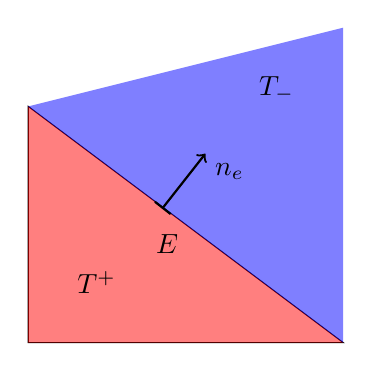
\begin{tikzpicture}[scale=1]
\coordinate (A) at (0,0);
\coordinate (C) at (0,3);
\coordinate (B) at (4,0);
\coordinate (D) at (4,4);
\coordinate (Tm) at (3.5,3.5);
\coordinate (Tp) at (0.5, 0.5);
\coordinate (e) at (1.5, 1.5);
\coordinate (start) at (1.7, 1.7);
\coordinate (end) at (2.25, 2.4);

\draw (A) -- (B) -- (C) -- cycle;
\fill[red, opacity=0.5] (A) -- (B) -- (C);
\fill[blue, opacity=0.5] (B) -- (C) -- (D);
\node[below left] at (Tm) {$T_{-} $ };
\node[above right] at (Tp) {$T^{+}$ };
\node[below right] at (e) {$E$ };

\draw [|->, thick] (start) -- (end);
% \node[above right] at (A) {A };
% \node[below right] at (B) {B};
% \node[above right] at (C) {C };
% \node[below right] at (D) {D};
\node[below right] at (end) {$n_e$};
\end{tikzpicture}
\caption{Edge $E \in \mathcal{F}_h $ shared by the triangles $T_{+}, T_{-} \in \mathcal{T}_{h} $ and the normal unit vector $n_{e}$.  }
    \label{fig:normal}
\end{figure}


Using the same method as in \cite{gu2012c0, brenner2012quadratic} can we
deduce that for every triangle $T \in  \mathcal{T}_{h} $ is \[
    \begin{split}
        \left( \nabla ^{4} w, v \right) _{T} &= \left< \partial _{n} \nabla ^2 w, v \right>_{\partial T} - \left( \nabla \left( \nabla ^2 w
 \right), \nabla  v  \right)_{T}   \\
 &= \left( D^2w, D^2v \right)_{T} + \left< \partial _{n} \nabla ^2 w, v \right>_{\partial T}  - \left<\partial _{n}
 \nabla w, \nabla v \right>_{\partial T} \\
 &=  \left( D^2 w, D^2 v \right)_{T} - \left<\partial _{nt} w, \partial _{t} v \right>_{\partial T} - \left<\partial
 _{nn} w, \partial _{n} v \right> _{\partial T} +  \left<\partial _{n} \nabla ^2 w, v \right>_{\partial T} \\
    \end{split}
\]
Keep in mind that this result naturally arise when defining $\nabla  = \left( \partial _{n}, \partial _{t} \right) $ such that
\[
\left<\partial _{n} \nabla w, \nabla v \right>_{\partial T} = \left<\partial _{nt} w, \partial _{t} v\right> _{\partial
T} + \left< \partial _{nn} w, \partial _{n} v  \right> _{\partial T} .
\]
 Thus, letting $u,v \in
H^{4}\left( T  \right) $  does this hold for local continuity,

\begin{equation}
\label{eq:bi_basic_dg}
\left( \nabla ^{4} u,v \right) _{T} = \left( D^2u,D^2v \right) _{T } - \left<\partial _{nt} u, \partial _{t}v
\right>_{\partial t} - \left<\partial _{nn} u, \partial _{n}v \right>_{\partial T} + \left<\partial _{n} \nabla ^2 u,v
\right>_{\partial T}
.\end{equation}

For global continuity does it end up with  so that $v \in \left\{ v \in H^{1}\left( \Omega  \right): v_{T} \in  H^{4}\left( T \right), \ \forall T \in
\mathcal{T}_{h}    \right\}   \cap C^{0} (
\overline{\Omega }  ) $ such that

\begin{equation}
\label{eq:bi_basic_dg_full_1}
\left( \nabla ^{4} u, v \right) _{\Omega }
= \sum_{T \in  \mathcal{T} _{h}}^{} \left( D^2u, D^2v \right)_{T}  + \sum_{E \in
\mathcal{F} ^{ext}_{}}^{} \left<\partial _{n} \nabla  ^2 u, v  \right> _{E}
- \left<\partial _{nt} u, \partial _{n} v \right> _{E}
+ \sum_{E \in \mathcal{F}  ^{int}}^{} \left<\partial _{nn} u , \jump{ \partial _{n_{e}} v }
\right>_{E}.
\end{equation}

What we see is that for \eqref{eq:bi_basic_dg} and \eqref{eq:bi_basic_dg_full_1} to be equivalent on normal and global form must this be true
\[
 \sum_{T \in  \mathcal{T}_{h} }^{}  - \left<\partial _{nt} u, \partial _{t}v
\right>_{\partial T} - \left<\partial _{nn} u, \partial _{n}v \right>_{\partial T} + \left<\partial _{n} \nabla ^2 u,v
\right>_{\partial T}
=  \sum_{E \in
\mathcal{F}^{ext}  }^{} \left<\partial _{n} \nabla  ^2 u, v  \right> _{E}
- \left<\partial _{nt} u, \partial _{n} v \right> _{E}
+ \sum_{E \in \mathcal{F}^{int} }^{} \left<\partial _{nn} u , \jump{ \partial _{n_{e}} v }
\right>_{E}
\]

%      Here is what is happening in Gu \cite{gu2012c0}. Let $w_{h}, v_{h} \in V_{h} = \left\{ v \in C\left(
%         \overline{\Omega }  \right): v_{T } = v \mid _{T} \in  \mathcal{P}   _{2} \left( T \right) \quad  \forall T \in
%     \mathcal{T}_{h} \right\} $.

% Anyhow, \textbf{assuming} that this equation holds can we introduce the numerical correction term,  \[
% \sum_{E \in  \mathcal{F} _{h}}^{}  \tau _{h} \left< \jump{ \partial _{n_{e}} w_{h}}, \jump{     \partial _{n_{e}} v_{h}
% }   \right>_{E}
% \]

% \todo[inline]{ Do some research on the correct stability and symmetry term and why this is necessarry.}
% Where $\tau _{h}$ is to be determined based on each triangulation.


Keep in mind that the jump is defined as $\jump{ \partial _{n_e} v _{h} } = n_{e} \left( \nabla v_{+} - \nabla v_{-}
\right)   $ and similarly will the mean be $\mean{ \partial_{  n_{e} } v_{h}  } = \frac{1}{2}n_{e}(   \nabla _{+ }v_{h})
+ \nabla _{-} v_{h}$ . We have now the final C0IP formulation.
The discretized numerical problem is to solve $w_{h} \in V_{h}$ such that \[
\mathcal{A}\left( w_{h}, v_{h} \right)   = F\left( v_{h} \right), \quad \forall v_{h} \in V_{h}  .
\]
where

\begin{equation}
\label{eq:basic_dg_A_h}
\begin{split}
\mathcal{A} \left( w_{h}, v_{h} \right)   =&
  \quad  \left( \beta \nabla w_{h} \cdot \nabla v_{h}  \right)_{\Omega } + \left( \gamma w_{h}, v_{h} \right) _{\Omega }\\
&  + \sum_{T \in \mathcal{T} _{h}}^{} \left( D^2 w_{h}, D^2v_{h} \right) _{T} \\
 & +
  \sum_{E \in \mathcal{F}_{h} }^{} \left<\mean{  \partial _{n_{e} n_{e}} w_{h} }, \jump{ \partial _{n_{e}} v_{h}}
\right>_{E}  + \left< \mean{ \partial _{n_{e} n_{e}} v_{h} }, \jump{ \partial _{n_{e}}w }      \right>_{E} + \tau _{h} \left< \jump{ \partial _{n_{e}} w_{h}}, \jump{ \partial _{n_{e}} v_{h}   }   \right>_{E} \\
\end{split}
\end{equation}
and
\begin{equation}
\label{eq:basic_dg_F_h}
F\left( v_{h} \right)  = \left( f, v_{h} \right) _{\Omega } - \left<q, v_{h} \right> _{\partial \Omega }
.\end{equation}
Notice that the regulation $\tau _{h}$ is to be determined by for every edge.

In \cite{gu2012c0} they introduce \[
            \begin{split}
    \left( D^2v: D^2w \right)_{T } & = \left<\partial _{nt} v , \partial _{t} w  \right>_{\partial T} + \left< \partial
    _{nn} v
    \partial _{n}, w \right>_{\partial T}. \\
    &= \sum_{i=1}^{3} \partial _{n_{i} t_{i}} v \int_{E_{i}}^{} \partial _{t} w ds +\left< \partial
    _{nn} v,
    \partial _{n} w \right>_{\partial T}     \\
    &=\left< \partial
    _{nn} v,
    \partial _{n} w \right>_{\partial T}  \\
            \end{split}
    \]
    Using the identity $ab +cd = \frac{1}{2} (a+c)(b+d) + \frac{1}{2}(a-c)(b-d) $  they end up with the equations  \[
    \sum_{T \in \mathcal{T}_{h}  }^{} \left( D^2v: D^2w \right)_{T }  =
    - \sum_{E \in \mathcal{F} ^{int}}^{}  \mean{ \partial _{n_e n_{e}} v  } \jump{ \partial _{n_{e}} w } - \jump{
    \partial _{n_e n_{e}} v}  \mean{ \partial _{n_{e}} w }
\]

\subsubsection{HC0IP Method copied from NGSolve}%
\label{ssub:hc0ip_method_from_ngsolve}

We consider the Kirchhoff plate equation: Find $w \in H^2$, such that

$$
\int \nabla^2 w : \nabla^2 v = \int f v
$$

A conforming method requires $C^1$ continuous finite elements. But there is no good option available, and thus there is no $H^2$ conforming finite element space in NGSolve.

$$
\sum_T \nabla^2 w : \nabla^2 v
- \int_{E} \{\nabla^2 w\}_{nn} \, [\partial_n v]
- \int_{E} \{\nabla^2 v\}_{nn} \, [\partial_n w] + \alpha \int_E  [\partial_n w]  [\partial_n v]
$$

[Baker 77, Brenner Gudi Sung, 2010]

We consider its hybrid DG version, where the normal derivative is a new, facet-based variable:

$$
\sum_T \nabla^2 w : \nabla^2 v
- \int_{\partial T} (\nabla^2 w)_{nn} \, (\partial_n v - \widehat{v_n})
- \int_{\partial T} (\nabla^2 v)_{nn} \, (\partial_n w - \widehat{w_n}) + \alpha \int_E (\partial_n v - \widehat{v_n}) (\partial_n w - \widehat{w_n})
$$
% Anyhow,
% let us first define the Hilbert space of the discrete solution \[
% \begin{split}
%     H^{1}\left( \mathcal{T}_{h}  \right)  & = \left\{ v \in L_{2} \left( \Omega  \right) : v  \mid _{T} \in H^{1} \left( T
%     \right) \forall T \in \mathcal{T}_{h}    \right\} \\
%     V &=  \left\{ v \in H^2\left( \Omega  \right) : \partial _{n} v = 0 \text{ and } \partial _{n} \nabla ^2 v = 0 \text{ on } \partial \Omega  \right\} \\
% \end{split}
% \]
% \todo[inline]{ Probably need to work more on this argumentation }

% Let us now define $u,v \in V$.

% \subsubsection{HDG Method}%
% \label{ssub:dg_method}
% Let us now define our workspace using the spaces

%  \[
% \begin{split}
%     V &=  \left\{ \left( u, u_{F}  \right): u \in H^{4}\left( \mathcal{T} _{h} \right) \cap H^{1}\left( \Omega  \right)   \right\} \\
%     V_{h} &=  \left\{ \left( u, u_{F}  \right) : u \in \mathcal{P} ^{k}\left( T \right) \forall T \in  \mathcal{T} ,
%     u_{F} \in \mathcal{P} ^{k}\left( E \right) \forall E \in  \mathcal{F}_{h}    \right\} \\
% \end{split}
% \]

% and the ones including the null drichlet conditions \[
% \begin{split}
%     V_{0} &= \left\{ \left( u, u_{F} \right) \in  V : \quad u =0, u_{F} = 0 \text{ on } \partial \Omega   \right\}, \\
%     V_{0,h} &= \left\{ \left( u, u_{F} \right) \in  V_{h} : \quad u =0, u_{F} = 0 \text{ on } \partial \Omega   \right\}
%    . \\
% \end{split}
% \]
% Let $\left( u, u_{F} \right) \in  V $\[
%     \begin{split}
% \sum_{T}^{} \left( \nabla ^{4} u,v \right) & = \sum_{T}^{} \left( \nabla ^{3} u, \nabla  v \right)_{T} + \left<\partial _{n}
% \nabla ^2 u, v \right>_{\partial \Omega } \\
% &= \sum_{T}^{} \left( \nabla ^2 u, \nabla ^2 v \right)_{T} - \left<\partial _{n} \nabla u, \nabla v \right>_{\partial T}
% + \left< \partial _{n} \nabla ^2 u, v \right> _{\partial T}\\
%     \end{split}
% \]




